%latexmk -pdf -pvc notes.tex
\documentclass{article}
\usepackage[utf8]{inputenc}

\title{Lectures notes of Distributed Algorithm on Shared memory}
\author{Garance Gourdel}
\date{September 2018}

\usepackage{natbib}
\usepackage{graphicx}
\graphicspath{{Pictures/}}


\usepackage{amsthm}
\usepackage[a4paper,top=3cm,bottom=2cm,left=3cm,right=3cm,marginparwidth=1.75cm]{geometry}

 
\theoremstyle{definition}
\newtheorem{definition}{Definition}[section]
\newtheorem{theorem}{Theorem}

\begin{document}

\maketitle
\tableofcontents

\section{Introduction}

Distributed algorithm is a crucial problem as some problems are just impossible to solve in sequential.
Overall there are two important laws that were significant in the understanding of the importance of Distributed algorithm.
\\
First, the Moore's law was that the number of transistors in a dense integrated circuit double every two year.
\begin{center}
	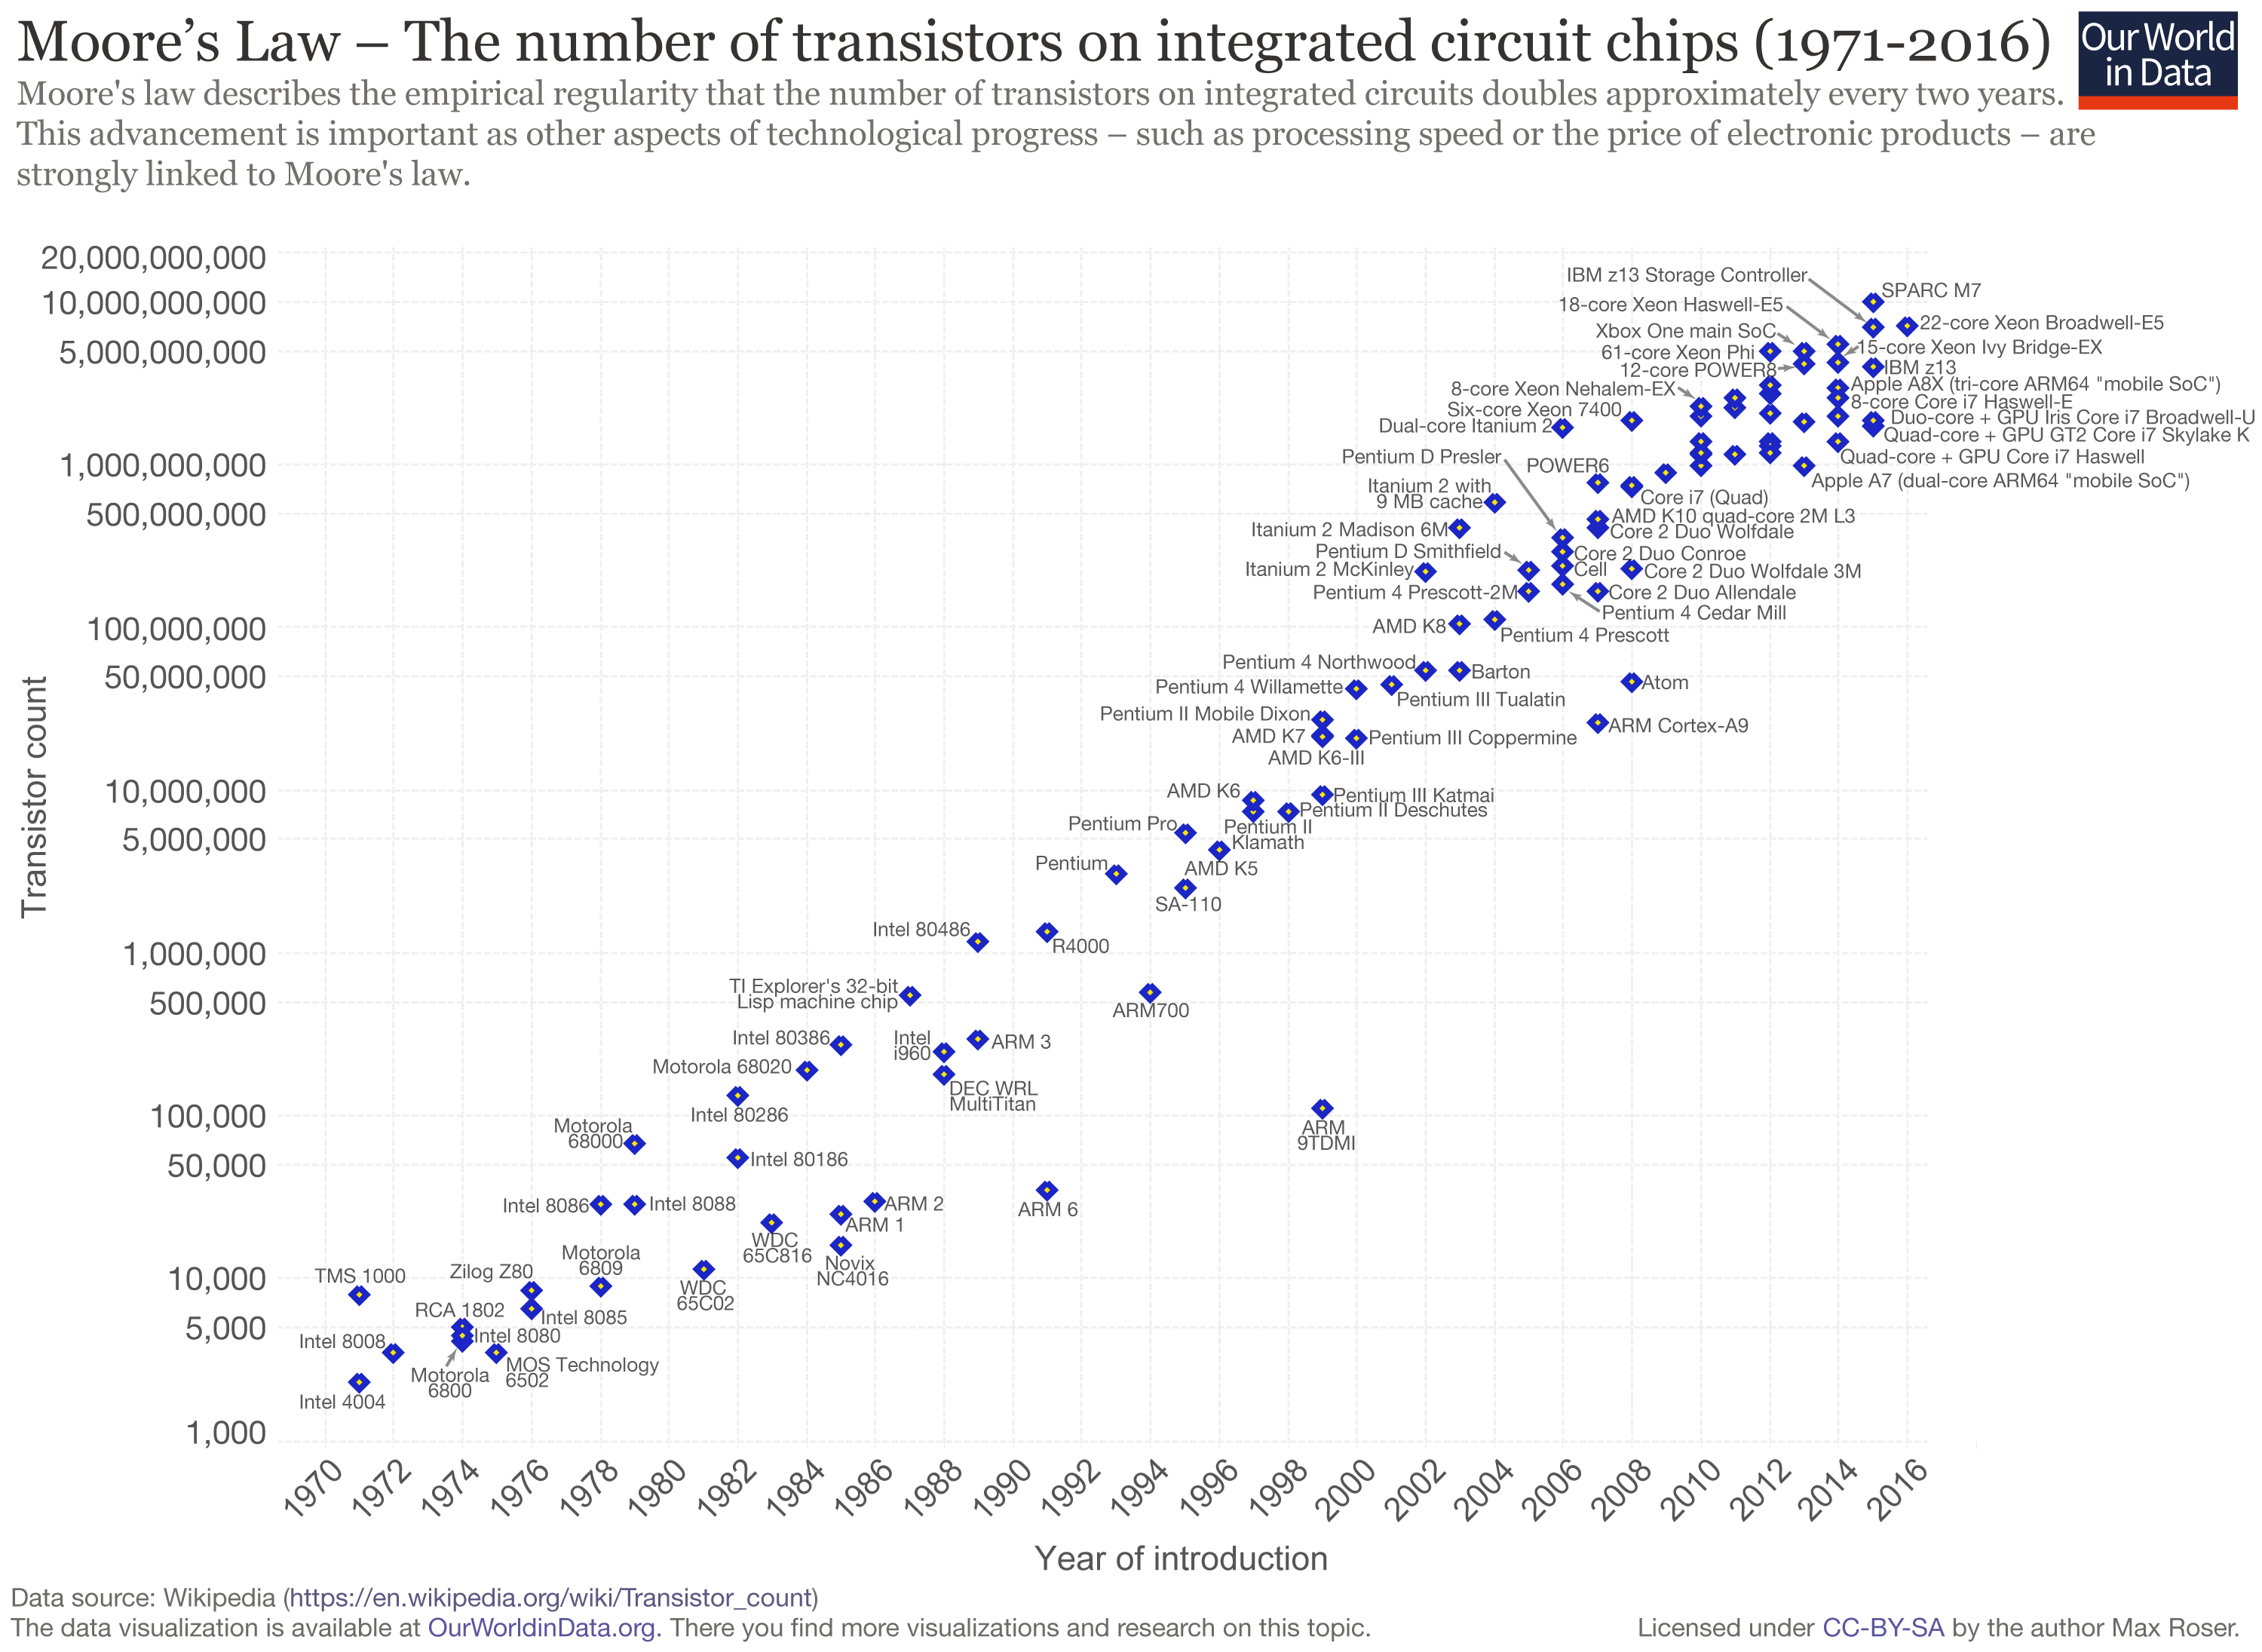
\includegraphics[width=0.8\textwidth]{Moore}
\end{center}
This improvement of the processors ended around the years 2003~2004. But the conclusion was that we could still add more cores to improve the performances.
\\

Then comes the Amdahl's law, it says that if $p$ is the fraction of work that can be done in parallel and $n$ the number of processors, and considering that each processors needs time 1 to complete the job, the speed up is : $$ \frac{1}{1- p + \frac{p}{n}} $$
Which can be summed up as "the cost of synchronization is high.

Synchronization is the coordination of every program and it takes time, asynchronicity at the opposite is random scheduling.

Something that is also important to understand is that Distributed algorithm and parallelization aren't the same thing, one considers that there is a supervisor (parallel) and the other one does not.
The main challenge in distributed computing is correctness, furthermore in distributed computing if a computer crashes, no computation can be done.

In conclusion, every system is now concurrent, every parallel program needs to synchronize and the cost of synchronization is high.

\vspace{0.5 cm}
{\Large \centering \textbf{Synchronization, blocking and non blocking}}
\vspace{-0.3 cm}

\section{Definition}

\begin{definition}{Mutual exclusion}
No two processes are in their critical sections (CS) at the same time.
\end{definition}

\begin{definition}{Deadlock-freedom}
At least one process eventually enters its CS. (Assuming no process blocks in CS or Entry section)
\end{definition}

\begin{definition}{Starvation-freedom}
Every process eventually enters its CS. (Assuming no process blocks in CS or Entry section)
\end{definition}

Those where originally implemented by reading an writing algorithm such as peterson's lock or  Lamport’s bakery algorithm, now it's currently handle in hardware (with mutex, semaphores).

\section{Peterson Lock}
\begin{center}
	\large{\textbf{Peterson's lock 2 processes}}\\
	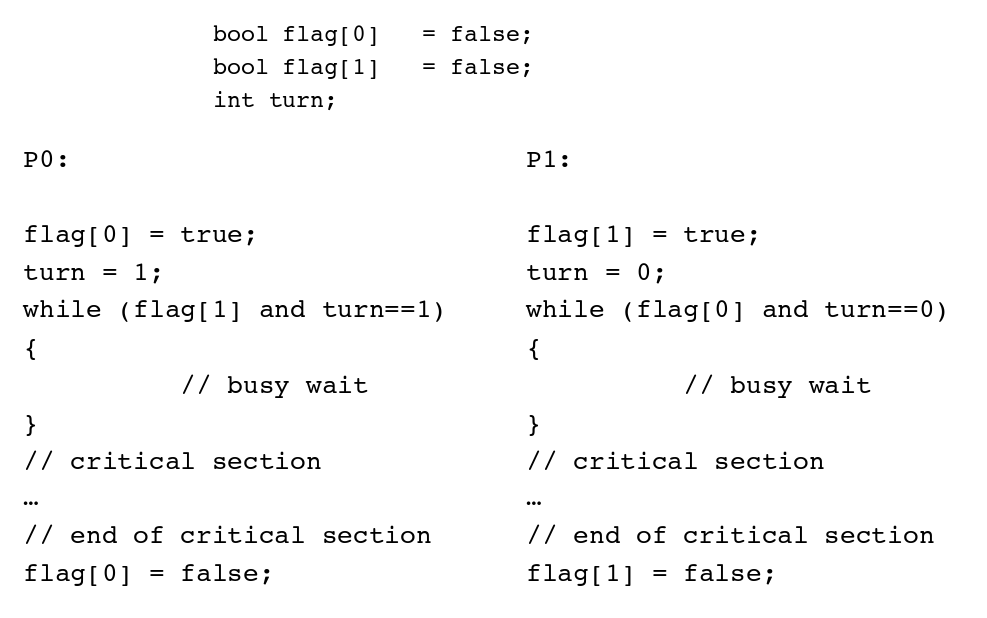
\includegraphics[width=0.8\textwidth]{peterson}
\end{center}

\begin{center}
	\large{\textbf{Peterson's lock N processes}}\\
	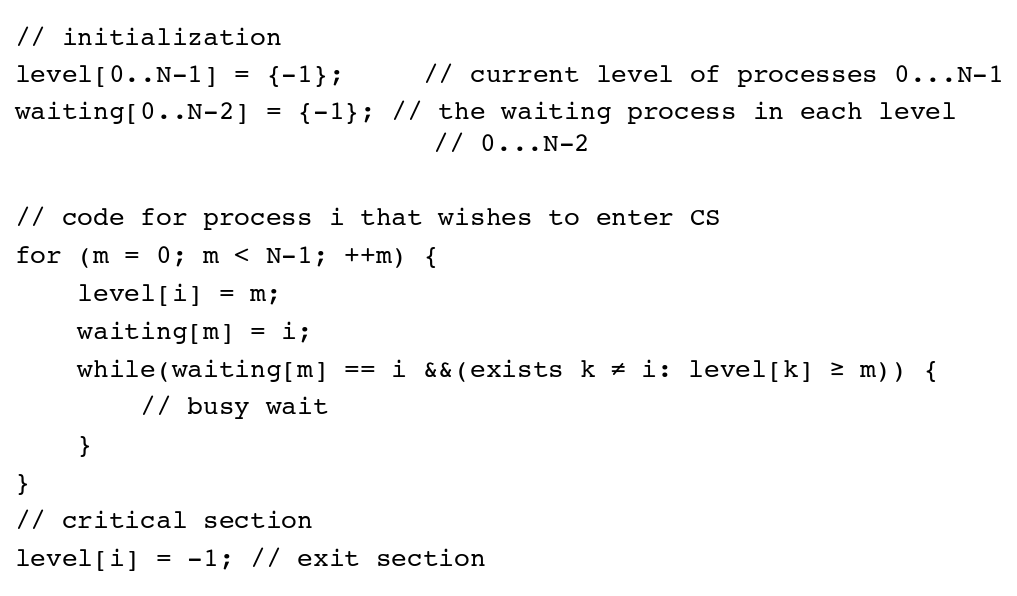
\includegraphics[width=0.8\textwidth]{peterson_N}
\end{center}

\begin{center}
	\large{\textbf{Bakery}}\\
	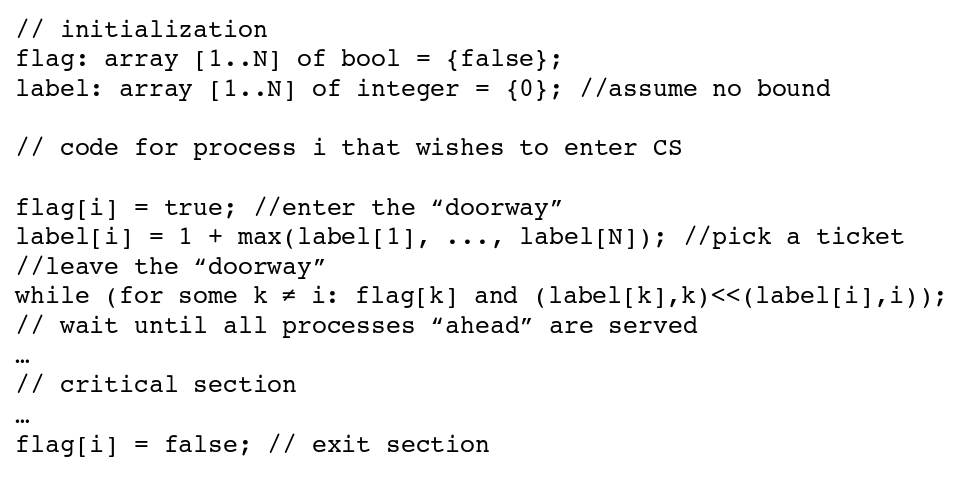
\includegraphics[width=0.8\textwidth]{bakery}\\
	Processes are served in the “ticket order”: first-come-first-serve.
\end{center}

\begin{center}
	\large{\textbf{Bakery simplified}}\\
	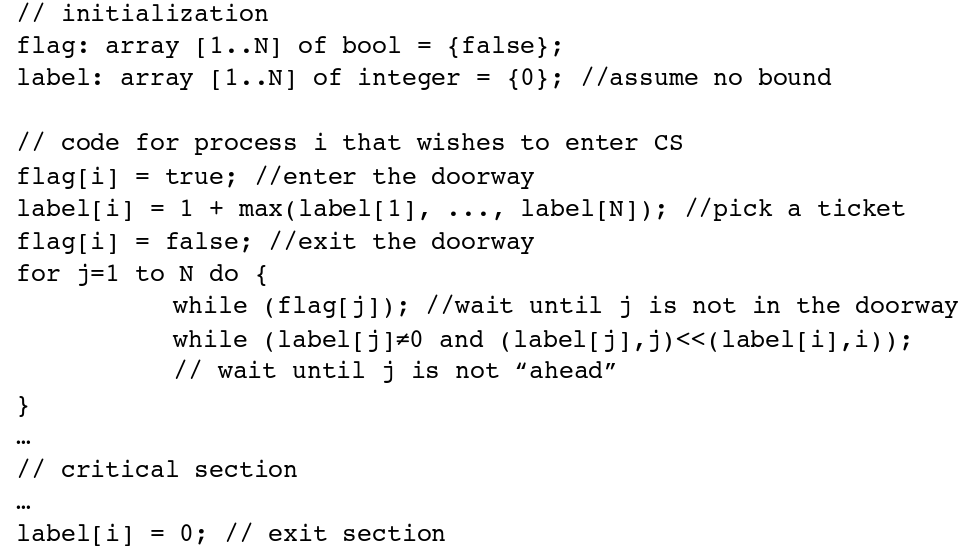
\includegraphics[width=0.8\textwidth]{bakery_2}\\
	Ticket withdrawal is "protected" with flags: a very useful trick: works with "safe" (non-atomic) shared variables.
\end{center}

\begin{center}
	\large{\textbf{Black and white Bakery}}\\
	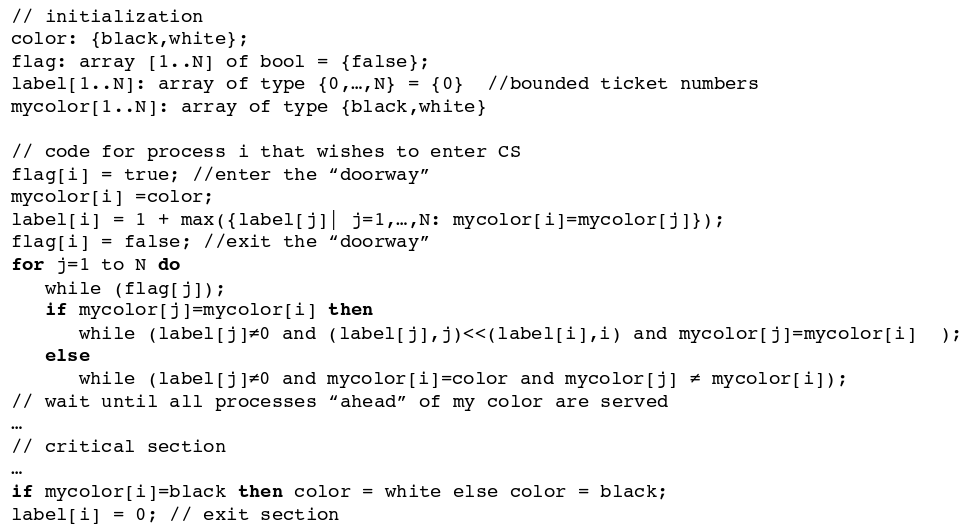
\includegraphics[width=0.8\textwidth]{bw_bakery}\\
	Colored tickets implies bounded variables!
\end{center}

\section{Synchronization tools}

\subsection{Readers-writers problem}
We have a writer and a reader, the writer updates a file and the reads keeps itself up-to-date but read and write are non-atomic. Synchronisation is necessary to make sure the reader doesn't read inconsistent values.
\begin{center}
	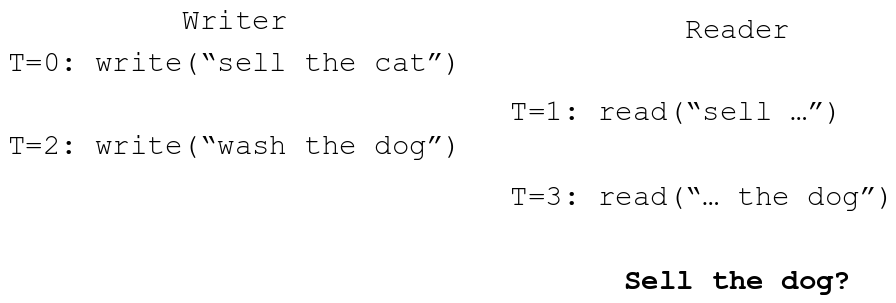
\includegraphics[width=0.8\textwidth]{read_writer_pb}
\end{center}

\subsection{Producer-consumer (bounded buffer) problem}

We have producers and consumers, Producers put items in the buffer (of bounded size), Consumers get items from the buffer. Every item is consumed, but no item is consumed twice, it is a very common situation : Client-server, multi-threaded web servers, pipes, ... Synchronisation is necessary to make sure items don't get lost and are not consumed twice.
\begin{center}
	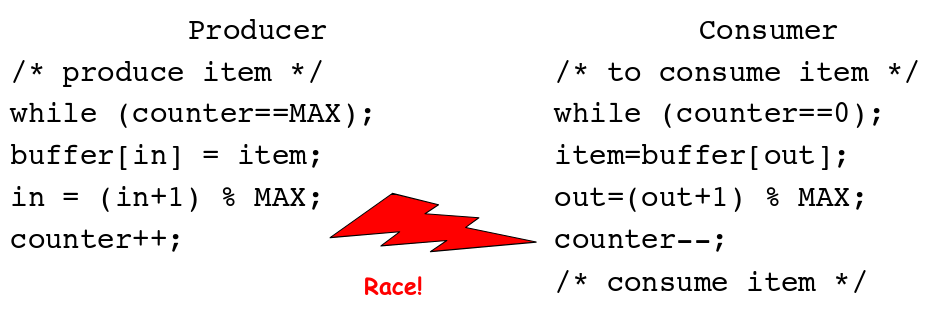
\includegraphics[width=0.8\textwidth]{producer_consumer_pb}
\end{center}

\subsection{Busy-wait: Test and Set}

\begin{definition}{Test and set}
$TAS(X)$ tests if $X = 1$, sets $X$ to 1 if not, and returns the old value of $X$.
\begin{center}
	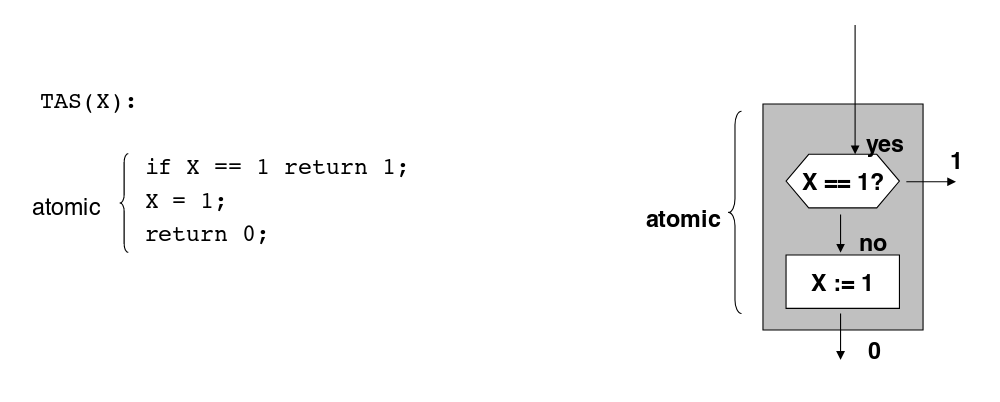
\includegraphics[width=0.8\textwidth]{TAS}
\end{center}
\end{definition}

But the problem is that the atomicity of the TAS is achieved by programs busy waiting, and for multiple producers and consumers we don't record the order of the requests.

\begin{center}
	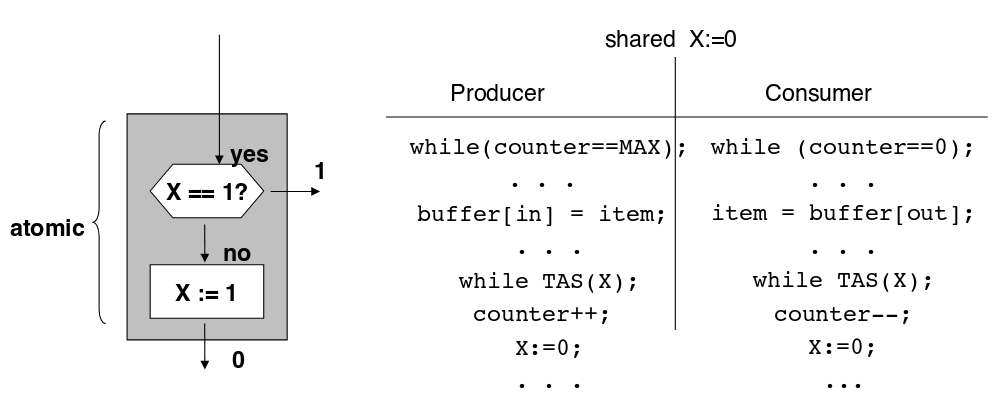
\includegraphics[width=0.8\textwidth]{TAS_busy_wait}
\end{center}

\subsection{Semaphores and locks}
\subsubsection{Semaphores}

\begin{definition}{Semaphores}
A semaphore $S$ is an integer variable accessed (apart from initialization) with two atomic operations $P(S)$ and $V(S)$ (Stands for “passeren” (to pass) and “vrijgeven” (to release) in Dutch).\\
The value of S indicates the number of resource elements available (if positive), or the number of processes waiting to acquire a resource element (if negative).
\begin{center}
	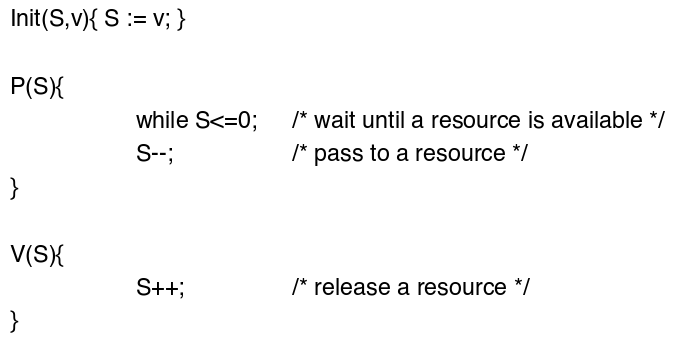
\includegraphics[width=0.6\textwidth]{semaphore}
\end{center}
\end{definition}

The implementation of a semaphore $S$ is a composite object: 
\begin{itemize}
	\item $S.counter$ the value of the semaphore.
	\item $S.wq$ the waiting queue, memorizing the processes having requested a resource element.
\end{itemize}

\begin{center}
\begin{tabular}{c c c}
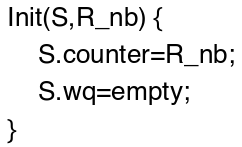
\includegraphics[width=0.2\textwidth]{sema_init} &
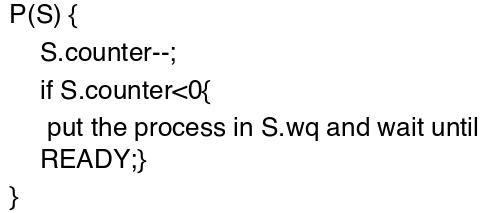
\includegraphics[width=0.4\textwidth]{sema_P} &
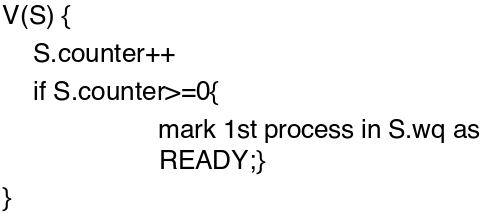
\includegraphics[width=0.4\textwidth]{sema_V}
\end{tabular}
\end{center}

\subsubsection{Locks}

\begin{definition}{Lock}
A semaphore initialized to 1, is called a lock (or a mutex). When a process is in a critical section, no other process can come in.
\begin{center}
	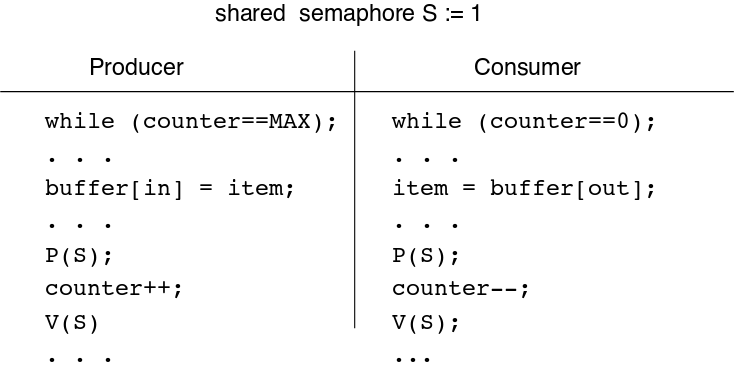
\includegraphics[width=0.6\textwidth]{lock}
\end{center}
\end{definition}

But we are, as mentioned before, still waiting until the buffer is ready.

\subsubsection{Semaphores for producer-consumer}

We can use 2 semaphores:
\begin{itemize}
	\item empty: indicates empty slots in the buffer (to be used by the producer)
	\item full: indicates full slots in the buffer (to be read by the consumer)
\end{itemize}
\begin{center}
	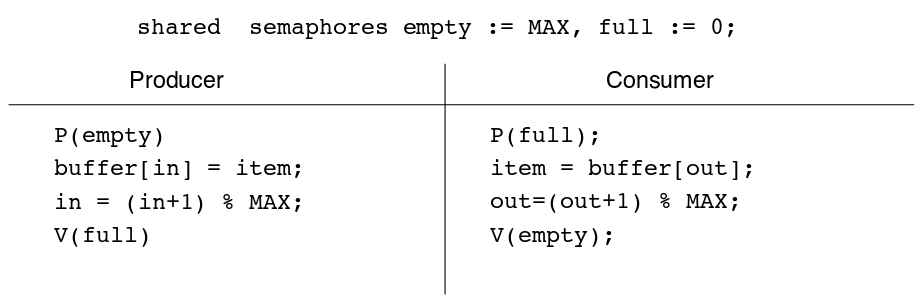
\includegraphics[width=0.8\textwidth]{sema_prod_consom}
\end{center}

\subsubsection{Problems of blocking synchronization}

With semaphores/locks we can have different problems:
\begin{itemize}
	\item Blocking: the progress of a process is conditional, it depends on other processes.
	\item Deadlock: no progress ever made
\begin{center}
	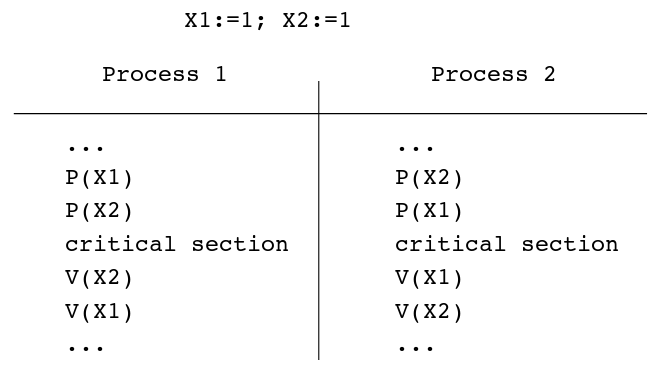
\includegraphics[width=0.5\textwidth]{pb_dead_lock}
\end{center}
	\item Starvation: requests blocked in the waiting queue forever
\end{itemize}

Overall blocking synchronization can cause priority inversion (High-priority threads blocked), Program not being robust (Page faults, cache misses etc) and not composable. Considering those problems could we think of anything else ?

\subsection{Nonblocking synchronization}
In such algorithm a process makes progress, regardless of the other processes, for example:
\begin{center}
	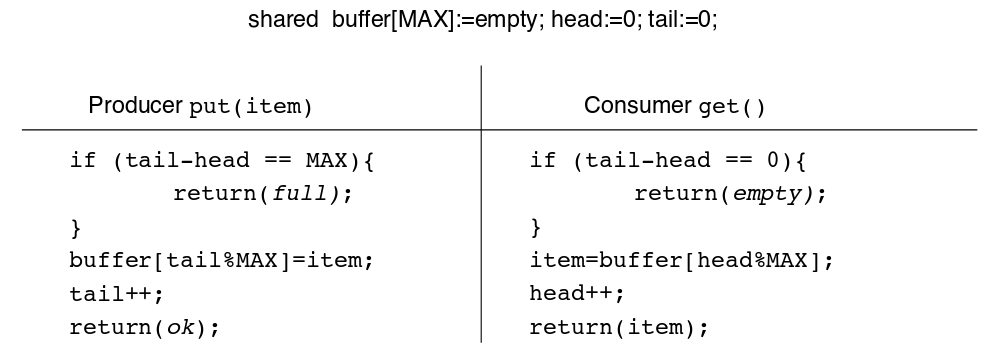
\includegraphics[width=0.8\textwidth]{non_block_prod_consom}
\end{center}

However, it works for 2 processes but it's hard to tell why it works, and how could we do for multiple producers or consumers, how could be apply to other synchronization problems ? We will investigate more those questions in the next sections of the course

\subsection{Transactional memory}
In this model, we have mark sequences of instructions as an atomic transaction, e.g., the resulting producer code:
\begin{center}
	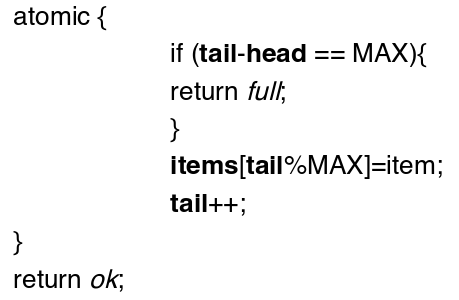
\includegraphics[width=0.4\textwidth]{prod_transactional}
\end{center}

Each transaction can be either committed or aborted:
\begin{itemize}
	\item Committed transactions are serializable
	\item Let the transactional memory (TM) care about the conflicts
	\item Easy to program, but performance may be problematic
\end{itemize}

%2ème séance
\section{Correctness of algorithms: Safety and Liveness}

Now if we want to continue in this path of analysing the system formally we have to define models (traceability, realism), devise abstractions for the system design  (convenience, efficiency), and devise algorithms and determine complexity bounds.

\begin{definition}
A \textbf{process} is an entity performing independent computation (this is an abstraction). The communication is made through message passing by \textbf{channel} and using a  shared memory \textbf{objects}.
\end{definition}

A process can be considered as automaton with states inputs outputs and a sequential specification.

An algorithm is a set of processes and can be either deterministic or randomized.

Processes communicate by applying operations on an receiving responses from \textit{shared objects}. Then a shared object instantiate a state machine with states, operations, responses and a sequential specification. We will see several examples of that : TAS, CAS, LL/SC ...

We are looking to implement an object, using base object, we aim to create an illusion that an object $O$ is available. 
\begin{center}
	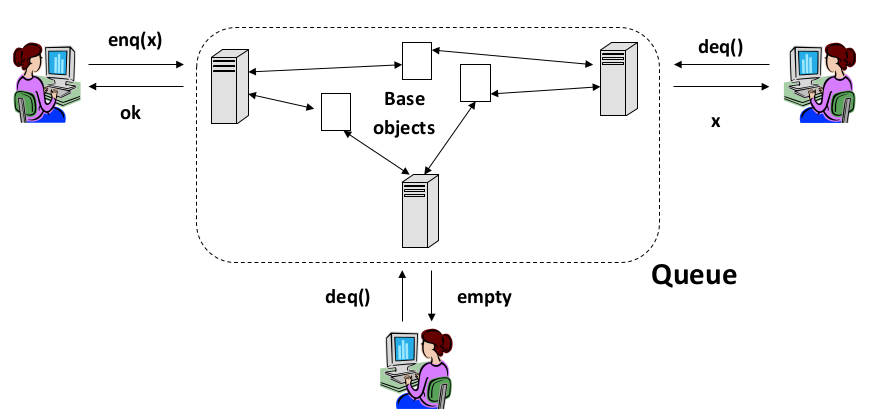
\includegraphics[width=0.8\textwidth]{queue_implem}
\end{center}

How can we define the correctness of an implementation ?

\subsection{Intuition}

Intuitively we define \textbf{Safety} as "noting bad ever happens". It can be violated in a finite execution, for example by producing a wrong output or sending an incorrect message. The question is "What the implementation is allowed o output ?"

Intuitively a \textbf{Liveness} property is "something good eventually happens. It can only be violated by an infinite execution, for example by never producing an expected output. And the question is under which condition the implementation outputs.

In our context, processes access abstractions by invoking operations. Operations are implemented by using sequences of accesses to base objects (for ex : a bounded-buffer using reads, writes, TAS, etc)

\begin{definition}
We say that a process is \textbf{correct} if it never fails (stop taking steps) in the middle of its operation.
\end{definition}

\begin{definition}
A system \textbf{run} is a sequence of events, for example actions that processes may take.
$\Sigma$ is the event's alphabet, for example all possible actions. and $\Sigma^{*\cup\infty}$ is the set of all finite and infinite runs.
\end{definition}

\subsection{Formal definitions}

\begin{definition}
A property $P$ is a \textbf{safety} property if :
\begin{itemize}
\item $P$ is \textbf{prefix-closed}: if $\sigma$ is in $P$, then each prefix of $\sigma$ is in $P$.
\item $P$ is \textbf{limit-closed}: for each infinite sequence of traces $\sigma_0$, $\sigma_1$, $\sigma_2$..., such that each $\sigma_i$ is a prefix of $\sigma_{i+1}$ and each $\sigma_i$ is in $P$, the limit trace $\sigma$ is in $P$. 
\end{itemize}
\end{definition}

\begin{definition}
$P$ is a \textbf{liveness} property if every \textbf{finite} $\sigma$ in $\Sigma^*$ has an \textbf{extension} in P.
\end{definition}

Note that it is enough to prove safety for all finite traces of an algorithm, and liveness for all infinite runs.

\subsection{Some examples}

We place our selves in a context where every processes \textbf{propose} values and \textbf{decide} on values. Determine whether the following are safety or liveness :
\begin{center}
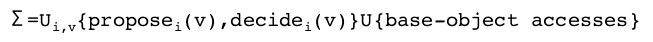
\includegraphics[width=\textwidth]{values.png}
\end{center}
And under the conditions that:
\begin{itemize}
\item Every decided value was previously proposed.
Safety.
\item No two processes decide differently.
Safety.
\item Every \textbf{correct} (taking infinity many steps) process eventually decides.
Liveness.
\item No two correct processes decide differently.
Liveness, it can not be determine in finite time whether a process is correct.
\end{itemize}

\subsection{Rules of thumb}

Let $P$ be a property:
\begin{itemize}
\item If every run that violates $P$ is \textbf{infinite} $\rightarrow$ $P$ is liveness.
\item Every run that violates $P$ has a finite prefix that violates $P$ $\rightarrow$ $P$ is safety.
\item Otherwise, P is a mixture of safety and liveness.
\end{itemize}

\section{Linearisability}

\subsection{Example implementing a concurrent queue}

We want to implement a concurrent FIFO queue but we are confronted with the fact that FIFO means strict temporal order, and concurrent implies an ambiguous temporal order.

By using a lock we immediately introduce a sequential behavior for the concurrency.

\begin{center}
\begin{tabular}{c c}
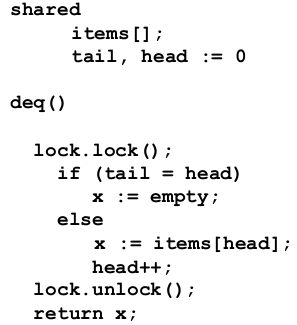
\includegraphics[width=0.3\textwidth]{FIFO_lock} &
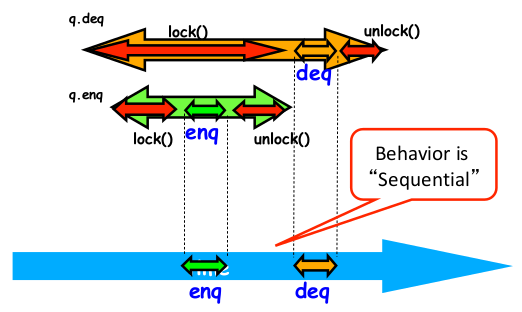
\includegraphics[width=0.5\textwidth]{FIFO_seq}
\end{tabular}
\end{center}

\subsection{linearizability and histories}

Linearizability is a Safety (and atomicity) property. Each operation should :
\begin{itemize}
\item "take effect"
\item Instantaneously
\item Between invocation and response events
\end{itemize}

On the thumb we can say that the history of a concurrent execution is correct if its "sequential equivalent" (it's history) is correct. Let us now define formally histories:

\begin{definition}
A \textbf{history} is a sequence of invocation and responses :\\ E.g. p1-enq(0), p2-deq(),p1-ok,p2-0,... \\
A history is \textbf{sequential} if every invocation s immediately followed by a corresponding response :\\ E.g., p1-enq(0), p1-ok, p2-deq(),p2-0,... \\
In particular a sequential history has no concurrent operations.
\end{definition}

\begin{center}
\begin{tabular}{c c}
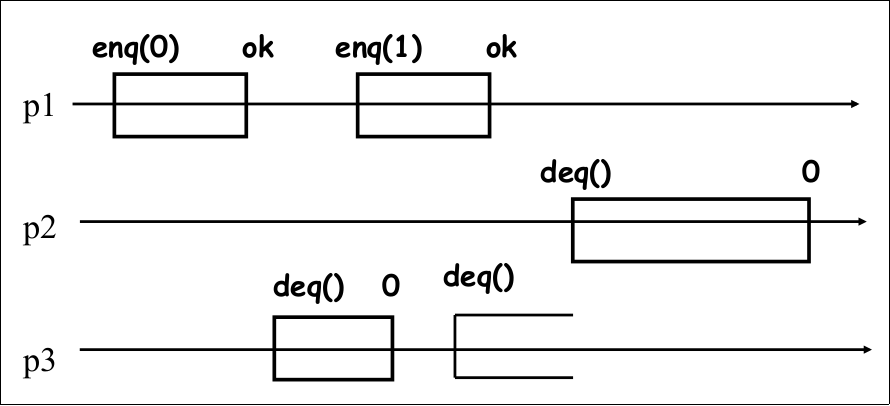
\includegraphics[width=0.5\textwidth]{history1}&
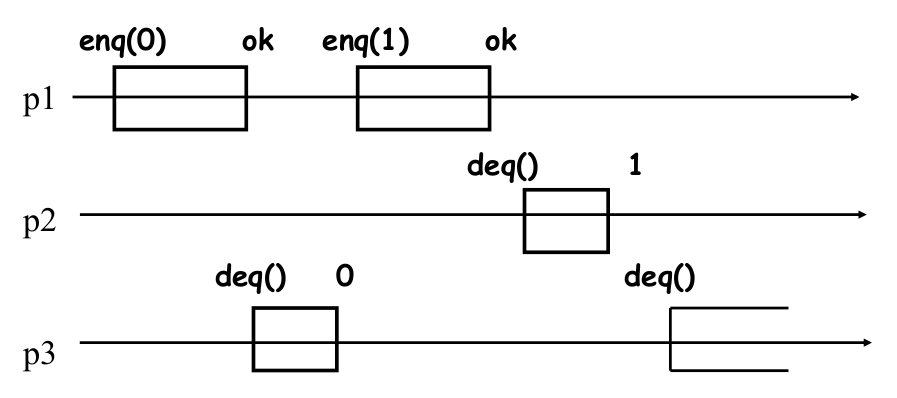
\includegraphics[width=0.5\textwidth]{history2}\\
\tiny{p1-enq(0); p1-ok; p3-deq(); p1-enq(1); p3-0; p3-deq(); p1-ok; p2-deq(); p2-0} &
\tiny{p1-enq(0); p1-ok; p3-deq(); p3-0; p1-enq(1); p1-ok; p2-deq(); p2-1;p3-deq();}
\end{tabular}
\end{center}

\begin{definition}
A sequential history is \textbf{legal} if it satisfies the sequential specification of the shared object.
\end{definition}

This definition translate for (FIFO) queues as : every deq returns the firs not yet dequeued value. And of Read-write registers : every read returns the last written value.

\subsection{completion}

\begin{definition}
Let $H$ be a history. AN operation $op$ is \textbf{complete} in $H$ if $H$ contains both the invocation and the response of $op$.\\
A \textbf{completion} of $H$ is a history $H'$ that includes all complete operations of $H$ and a subset of incomplete operations of $H$ followed with the matching responses.
\end{definition}

For the same history there are several completion possible :

\begin{center}
\begin{tabular}{c c c}
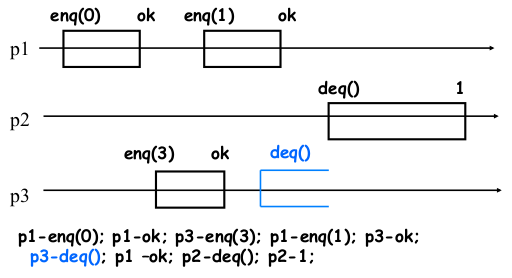
\includegraphics[width=0.3\textwidth]{complet_1}&
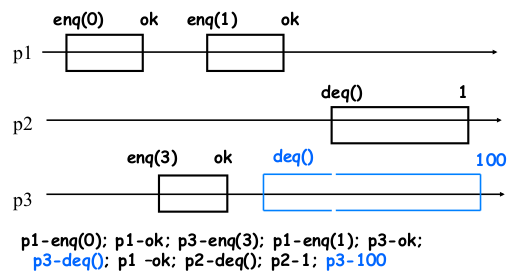
\includegraphics[width=0.3\textwidth]{complet_2}&
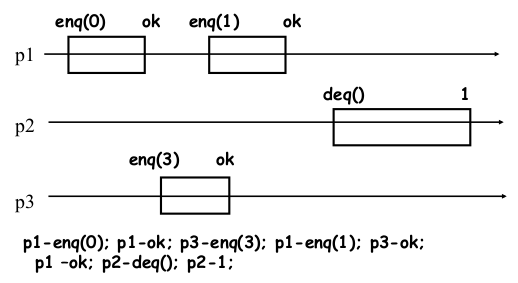
\includegraphics[width=0.3\textwidth]{complet_3}
\end{tabular}
\end{center}

\begin{definition}
Histories $H$ and $H'$ are \textbf{equivalent} if for all process $p_i$, $ H|_{p_i} =  H'|_{p_i} $.
\end{definition}

Examples : $H=p_1-enq(0); p_1-ok; p_3-deq(); p_3-3$ and $H’=p_1-enq(0); p_3-deq(); p_1-ok; p_3-3$

\begin{definition}\textbf{linearizability/atomicity}\\
A history $H$ is \textbf{linearizable} if there exists a \textbf{sequential legal} history $S$ such that:
\begin{itemize}
\item $S$ is \textbf{equivalent} to some completion of H.
\item $S$ preserves the \textbf{precedence relation} of $H$:
\begin{center}
$op1$ precedes $op2$ in $H$ $\rightarrow$ $op1$ precedes $op2$ in $S$
\end{center}
\end{itemize}
\end{definition}

\subsection{linearisation points}

\begin{definition}\textbf{linearizable}\\
An implementation is \textbf{linearizable} id every history it produces is linearizable.
\end{definition}

Informally we can view this as the fact that all operations (and some incomplete operation) in a history are seen as taking effect instantaneously at sometime between their invocation and responses. Operation are then ordered by their \textbf{linearization points} and must constitute a legal (sequential) history.

It here is are some examples of linearazitation, legal for 1 and 3 and illegal for 2 :
\begin{center}
\begin{tabular}{c c c}
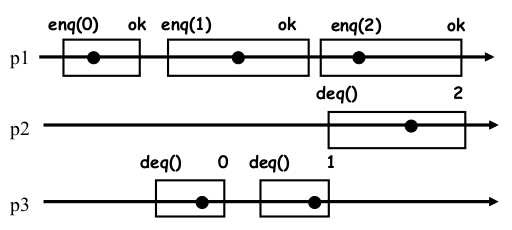
\includegraphics[width=0.3\textwidth]{linear_1}&
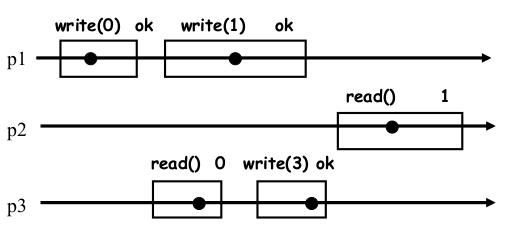
\includegraphics[width=0.3\textwidth]{linear_2}&
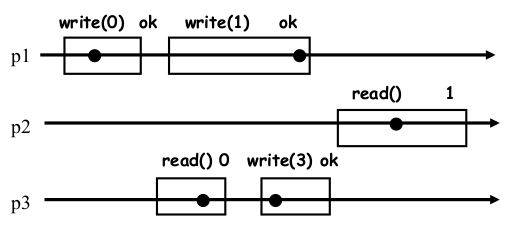
\includegraphics[width=0.3\textwidth]{linear_3}
\end{tabular}
\end{center}

But some history can't be linearized at all :
\begin{center}
\begin{tabular}{c c}
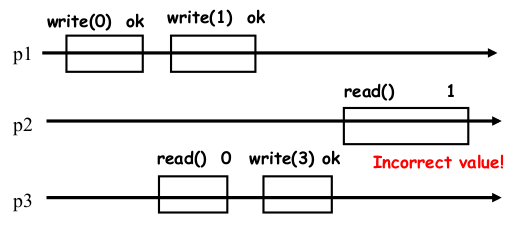
\includegraphics[width=0.3\textwidth]{linear_4}&
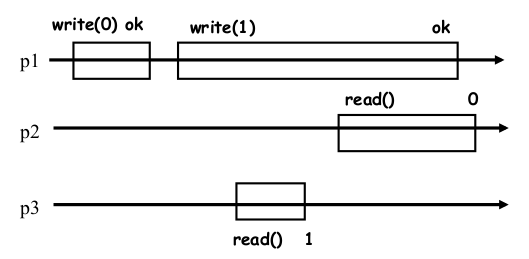
\includegraphics[width=0.3\textwidth]{linear_5}
\end{tabular}
\end{center}

And some can be linearized because they are incomplete :
\begin{center}
\begin{tabular}{c c}
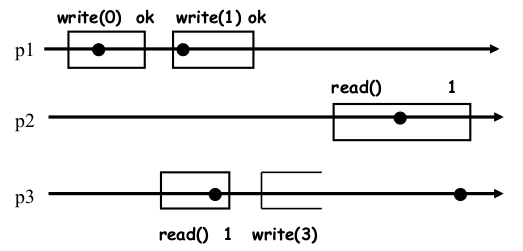
\includegraphics[width=0.3\textwidth]{linear_6}&
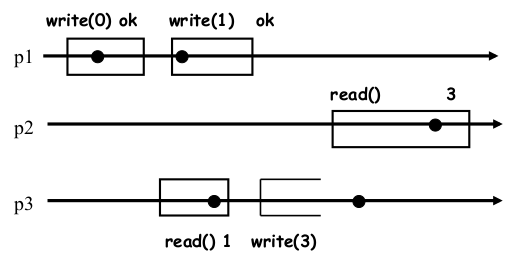
\includegraphics[width=0.3\textwidth]{linear_7}
\end{tabular}
\end{center}

We can also define \textbf{Sequential consistency} as : a history $H$ is \textbf{sequentially consistent} if there exists a \textbf{sequential legal} history $S$ such that :
\begin{itemize}
\item $S$ is \textbf{equivalent} to some completion of H.
\item $S$ preserves the \textbf{per(process order} of $H$:
\begin{center}
$p_i$ executes $op1$ before $op2$ in $H$ $\rightarrow$ $p_i$ executes $op1$ before $op2$ in $S$
\end{center}
\end{itemize}

But it's far less interesting as \textbf{linearizability is compositional} : Any history on two linearizable objects $A$ and $B$ is a history of a linearizable $composition(A,B)$. For example A composition of two registers $A$ and $B$ is a two-field $register(A,B)$. Where as sequential consistency is not, a composition of sequential consistent objects is not always sequential consistent.

\begin{center}
\begin{tabular}{c c}
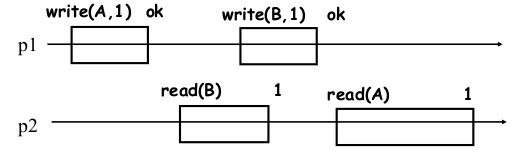
\includegraphics[width=0.4\textwidth]{compos}&
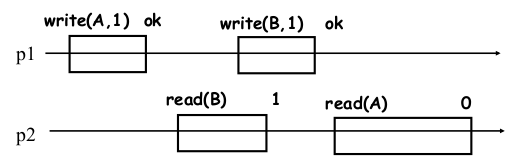
\includegraphics[width=0.4\textwidth]{not_compos}
\end{tabular}
\end{center}

Every incomplete operation in a finite history can be independently  : \textbf{Linearizability is nonblocking}.

Linearizability is a safety property :
\begin{itemize}
\item Prefix-closed: every prefix of a linearizable history is linearizable
\item Limit-closed: the limit of a sequence of linearizable histories is linearizable
\end{itemize}
And (see section 5) implementation is linearizable if and only if all its finite histories are linearizable.

Here it is good to think again why we wish to design linearizable objects and not just use a lock. Using a lock is simple it is an automatic transformation of the sequential code, it is correct, we get linearizability for free. On the other hand In the best case we get starvation freedom "if the lock is “fair” and every process cooperates, every process makes progress" but it is not robust to failures/asynchrony and trying to improve that with Fine-grained locking is complicated and prone to deadlocks.

\section{Liveness proprieties}

\subsection{definition}

Let us know define several liveness properties :
\begin{itemize}
\item Deadlock-free:If every process cooperates (takes enough steps), some process makes progress.
\item Starvation-free: If every process cooperates, every process makes progress.
\item Lock-free ( sometimes called non-blocking): Some active process makes progress.
\item Wait-free: Every active process makes progress.
\item Obstruction-free: Every process makes progress if it executes in isolation.
\end{itemize}

We can also sort them in a sort of "periodic" table of liveness properties:

\begin{center}
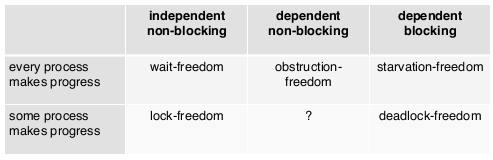
\includegraphics[width=0.8\textwidth]{periodic}
\end{center}

\subsection{hierarchy}

We can define relations between liveness properties as follows :
\begin{definition}
Property $A$ is \textbf{stronger} than property $B$ if every run satisfying $A$ also satisfies $B$ ($A$ is a subset of $B$).
$A$ is \textbf{strictly stronger} than $B$ if, additionally, some run in $B$ does not satisfy $A$, i.e., $A$ is a proper subset of $B$.
\end{definition}

For example:
\begin{itemize}
\item WF is stronger than SF \\
Every run that satisfies WF also satisfies SF: every correct process makes progress (regardless whether processes cooperate or not).
WF is actually strictly stronger than SF.
\item SF and OF are incomparable (none of them is stronger than the other)\\
There is a run that satisfies SF but not OF: the run in which $p1$ is the only correct process but does not make progress.
There is a run that satisfies OF but not SF: the run in which every process is correct but no process makes progress
\end{itemize}

%3eme séance

One interesting thing about linearization, is that from a model that gives us no guarantees in case of failures can also be transform into a model that will give us guarantees.

\section{Shared memory model}
On this model every processes communicates by applying operations on and receiving responses from shared objects.\\
A shared object is a state machine, with states, operations, responses and sequential specification. For example \textbf{read-write registers}, TAS, CAS, LLSC, ...

\begin{center}
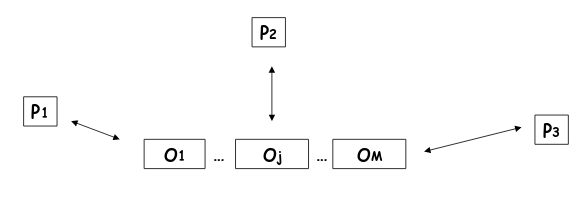
\includegraphics[width=0.8\textwidth]{sharedmemmodel}
\end{center}

\subsection{Readwrite register}

They can store values (in a value set $V$) an export two operations : read and write.
\begin{itemize}
	\item Write takes an argument in $V$ and returns ok.
	\item Read takes no arguments and returns a value in $V$.
\end{itemize}

Processes invoke operations on the shared objects and they may want some guarantees:
\begin{itemize}
	\item \textbf{Liveness}: the operations eventually return something
	\item \textbf{Safety}: the operations never return anything incorrect
\end{itemize}

%missing from slide 5 to 12~
Let us note what objects we will consider in this class, all objects considered in this class are wait-free and we only consider well-formed runs: a process never invokes an operation before returning from the previous invocation.

\begin{center}
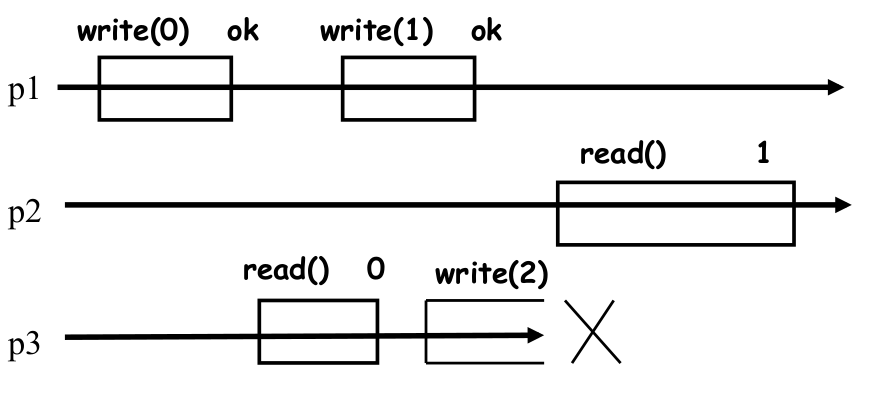
\includegraphics[width=0.6\textwidth]{well_formed}
\end{center}

\begin{definition}
\begin{itemize}
	\item Operation $op1$ \textbf{precedes} operation $op2$ in a run $R$ if the response of $op1$ precedes (in global time) the invocation of $op2$ in $R$.
	\item If neither $op1$ precedes $op2$ nor $op2$ precedes $op1$ than $op1$ and $op2$ are \textbf{concurrent}
\end{itemize}
\end{definition}

\subsection{Safety criteria}

As a reminder, we can say informally that safety implies that every read operation returns the “last” written value (the argument of the “last” write operation).

\begin{definition}{safe, regular and atomic registers}
\textbf{Safe registers} : every read that does not overlap with a write returns the last written value. \\
\textbf{Regular registers} : every read returns the last written value, or the concurrently written value. \\ 
\textbf{Atomic registers} : the operations can be totally ordered, preserving legality and precedence (linearisability). if read1 returns $v$, read2 returns $v^{'}$ and read1 precedes,read2, then write($v^{'}$) cannot precede write($v$) 
\end{definition}

\begin{center}
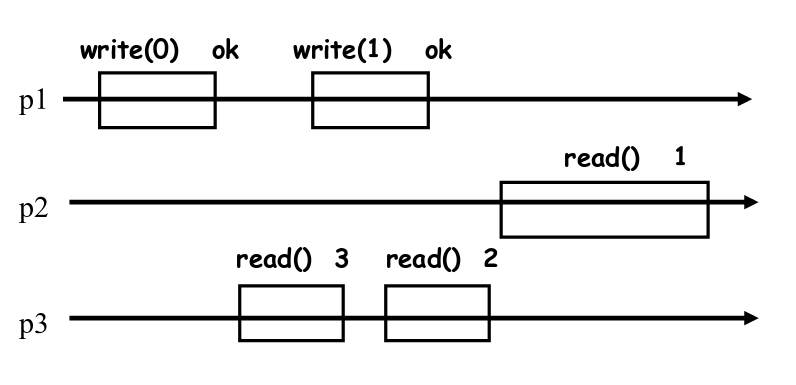
\includegraphics[width=0.8\textwidth]{c3_p1}\\
Safe register.
\end{center}

\begin{center}
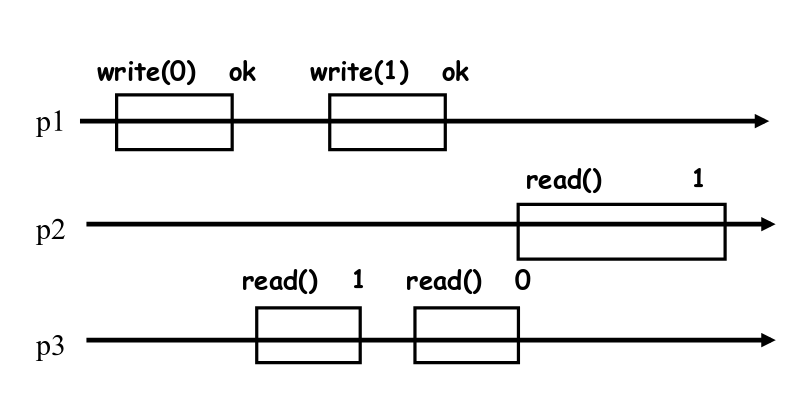
\includegraphics[width=0.8\textwidth]{c3_p2}\\
Regular register: this is not linearisable.
\end{center}

\begin{center}
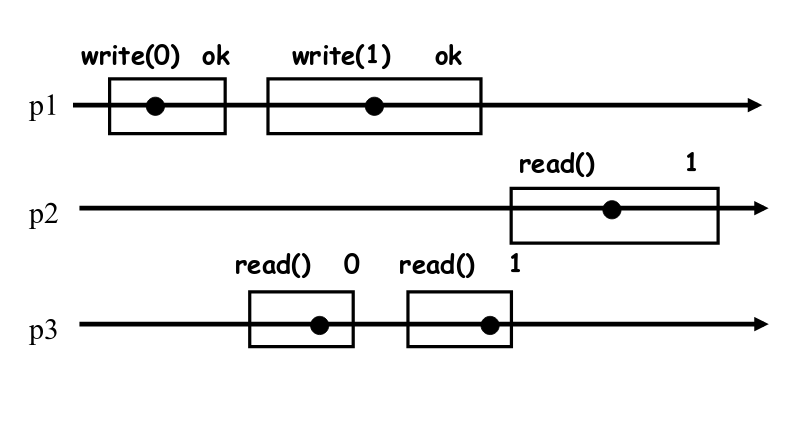
\includegraphics[width=0.8\textwidth]{c3_p3}\\
Atomic register: this is linearisable.
\end{center}

%Transformations slides 16 - 20 ~

\subsection{Transformation}

Let us consider how we define our registers. There are values either binaries or multi-valued. The number of readers anr writers : from 1-writer 1-reader (1W1R) to multi-writer multi-reader (NWNR). And finally the safety criteria: from safe to atomic.

\begin{theorem}
1W1R binary safe registers can be used to implement an NWNR multi-valued atomic registers!
\end{theorem}

\subsubsection{1WNR safe to 1WNR regular}

\begin{center}
\begin{tabular}{c c}
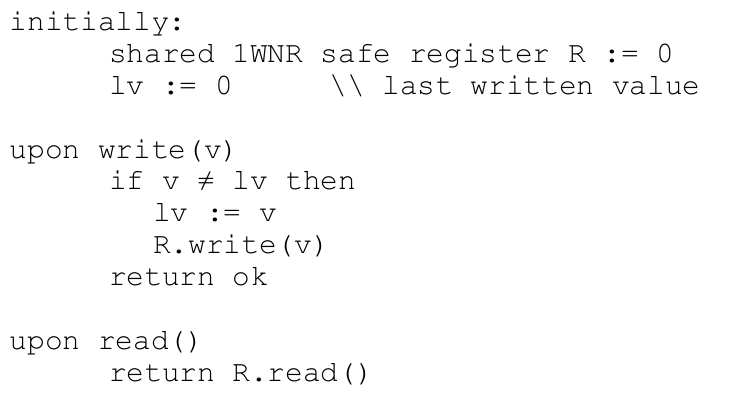
\includegraphics[width=0.5\textwidth]{transfo1}&
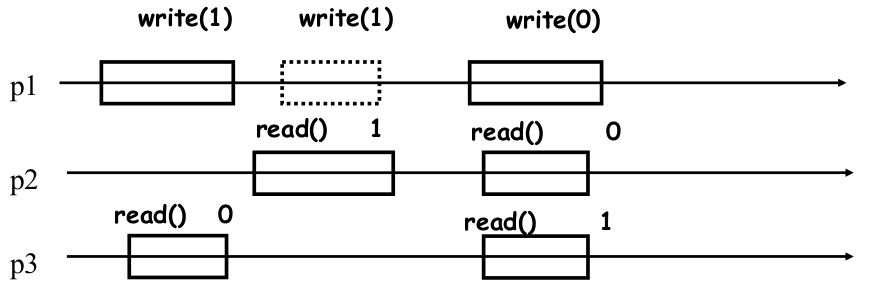
\includegraphics[width=0.5\textwidth]{transfo1_des}
\end{tabular}
\end{center}

\subsubsection{1W1R regular to 1WNR regular}

The registers can be either binary or multi-valued, but the proof is for binary.Let p1 be the only writer and 0 be the initial value.

\begin{center}
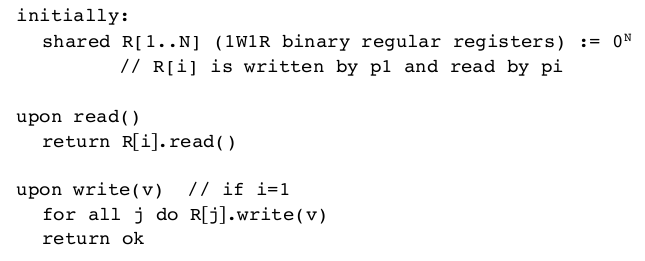
\includegraphics[width=0.5\textwidth]{transfo2}
\end{center}

\subsubsection{from binary to multi valued 1WNR}

\begin{center}
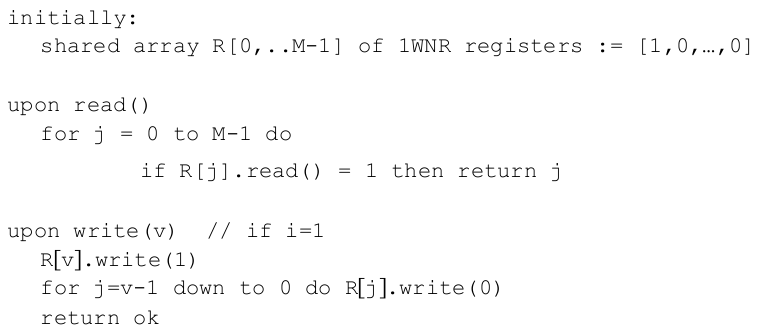
\includegraphics[width=0.5\textwidth]{transfo3}
\end{center}

\subsubsection{regular to atomic (1W1R)}

\begin{center}
\large{\textbf{Timestamps!}}\\
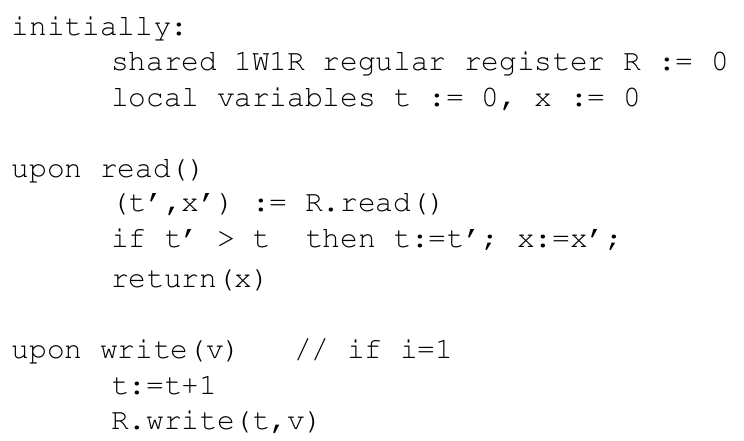
\includegraphics[width=0.5\textwidth]{transfo4}
\end{center}

\subsubsection{From 1W1R to 1WNR (multi-valued atomic)}

\begin{center}
\begin{tabular}{c c}
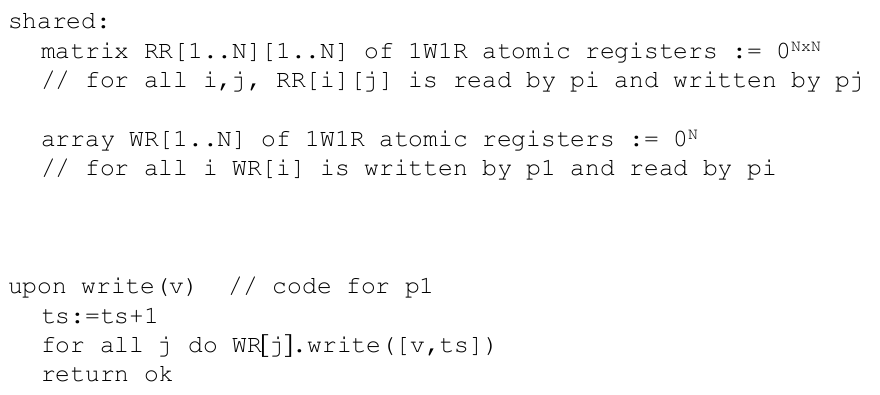
\includegraphics[width=0.5\textwidth]{transfo5}&
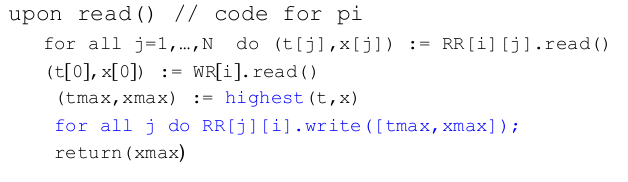
\includegraphics[width=0.5\textwidth]{transfo5_2}
\end{tabular}
\end{center}

%4eme scéance

\section{Atomic snapshot}

In the previous section, we saw that every registers, independently from their number of readers/writers, it's value set and safety property, all registers are (computationally) equivalent.

\begin{definition}{Atomic snapshot}
Its is a new object, reading multiple location atomatically, like a snapshot of all registers. Write to one, read to all.
\end{definition}

We can define a sequential specification, each process $p_i$ is provided with operation :
\begin{itemize}
	\item $update_i(v)$ returns ok
	\item $snapshot_i()$ returns $[v_1, ... , v_n]$
\end{itemize}
In this sequential execution, for each $[v_1, ... , v_n]$ returned by $snapshot_i()$, $v_j$ ($j=1...N$) is the argument of the last $update_j(.)$ (or the initial value if no such update)

\begin{center}
	\large{\textbf{Snapshot for free ?}}\\
	Code for process $p_i$:\\
	\includegraphics[width=0.8\textwidth]{snapshot_free}\\
	\vspace{0.5 cm}
	\large{\textbf{Problem!}}\\
	\includegraphics[width=0.8\textwidth]{snapshot_free_1}\\
	\vspace{0.5 cm}
	\includegraphics[width=0.8\textwidth]{snapshot_free_2}\\
\end{center}

The difficulty comes from having 3 or more processes. But what about lock-free snapshots ? \\
At least one correct process makes progress (completes infinitely many operations).

Code for process $p_i$ (all written values, including the initial one, are unique, e.g., equipped with a sequence number) :

\begin{center}
\includegraphics[width=0.8\textwidth]{lock_free_snapshot}\\
\end{center}

This can be linearized by assigning a linearization point to each operation:
\begin{itemize}
	\item $update_i(v)$ $R_i.write(v)$ if present, otherwise remove the op.
	\item $snapshot_i()$ if complete - any point between identical scans, otherwise remove the op.
\end{itemize}
It builds a \textbf{sequential history S} in the order of linearisation points.
S is legal: every $snapshot_i()$ returns the last written value for every $p_j$.\\
proof : Suppose not: $snapshot_i()$ returns $[x_1,...,x_N]$ and some $x_j$ is not the the argument of the $last update_j(v)$ in $S$ preceding $snapshot_i()$.\\

Let $C_1$ and $C_2$ be two scans that returned $[x_1,...,x_N]$, then :

\begin{center}
\includegraphics[width=0.8\textwidth]{lin_lock_free_snapshot}\\
\end{center}

%What can we do to make it wait free ? 

%Add slide 13 on lock-freedom if base registers are regular than the registers are not atomic and we can't necesarly linearized the snapshots.

Let's proove correctness: lock-freedom. Suppose a process $p_i$  execution $snapshot_i()$ eventually runs in isolation (no process takes steps concurrently). Then all scan received by $p_i$ are distinct, which means at least one process performs an update between. As there are finitely many processes, there is at least one process executes infinitely many updates.

What can we do to make it wait free ? You have to accept that an concurrent process writes while your snapshots. Then make the update do the work.

\begin{center}
\begin{tabular}{c c}
\includegraphics[width=0.4\textwidth]{code_gen_snap} &
\includegraphics[width=0.2\textwidth]{code_gen_upd} \vspace{\fill}
\end{tabular}
\end{center}

But of two scans differ, some update succeeded ! Would this work ?

\begin{center}
\large{\textbf{No!}}\\
\includegraphics[width=0.8\textwidth]{wait_free_snap_lin}\\
\end{center}

We can fix that : \textbf{If a process moved twice: its last snapshot is valid!}
\begin{center}
\includegraphics[width=0.8\textwidth]{wait_free_snap_lin_corr}\\
\end{center}

We claim that the complexity  is in $O(N^2)$ steps and it is wait free. This implementation is also linearizable : for update when write, for snapshot if there is two identical scans, then between the scans. Otherwise, if returned $U$ of $p_j$ : at the linearization point of $p_j$ ’s snapshot.

The linearization is legal : every snapshot operation returns the most recent value for each proces. But also consistent with the real-time order: each linearization point is within the operation’s interval and equivalent to the run (locally indistinguishable).

\section{One-shot atomic snapshot (AS)}

\begin{definition}
For one-shot atomic snapshot the snapshots can only be done after an update. Each process does $update_i(v_i )$, then a snapshot that returns $S_i$ .
\end{definition}

\begin{theorem}
We have that $v_i \in S_i$ (inclusion), and for all $i$ and $j$, $S_i$ is a subset of $S_j$ or $S_j$ is a subset of $S_i$ (containment).
\end{theorem}

\begin{center}
\begin{tabular}{c c}
\includegraphics[width=0.5\textwidth]{repres1} &
\includegraphics[width=0.5\textwidth]{repres2} 
\end{tabular}
\end{center}

\begin{definition}
For one-shot \textbf{immediate} atomic snapshot the snapshots can only be done after an update. Each process does $update_i(v_i )$, then a snapshot that returns $S_i$ , such that (\textbf{Immediacy}) for all $i$ and $j$: if $v_i$ is in $S_j$ , then $S_i$ is a subset of $S_j$.
\end{definition}

Then the representation is a subdivision : 
\begin{center}
\includegraphics[width=0.5\textwidth]{repres_is}\\
\end{center}

\begin{theorem}
IS is equivalent to AS (one-shot not immediate).
\end{theorem}

It is obvious that IS is a restriction of the AS, therefore IS is stronger than one-shot AS. A few one-shot AS objects can be used to implement IS :
\begin{center}
\includegraphics[width=0.8\textwidth]{implem_is}\\
\end{center}

Let's prove by induction correctness and that the algorithm satisfies Self-Inclusion, Snapshot, and Immediacy. The case $N=1$ is trivial.Suppose the algorithm is correct for $N-1$ processes. Then $N$ processes come to level $N$, at least one process returns in level $N$, by induction all properties hold of the ones that goes to level $N-1$. The process that return at level $N$ returns all $N$ values, thus all proporeties hold for all $N$ processes !

We define now \textbf{iterated immediate} snapshots (IIS) and shox it's representation over the number of iteration. First the iterated standard chromatic subdivision (ISDS), then one round of ISS then two round.
\begin{center}
\includegraphics[width=0.6\textwidth]{iis}\\
\begin{tabular}{c c c}
\includegraphics[width=0.3\textwidth]{iss_0} &
\includegraphics[width=0.3\textwidth]{iss_1} &
\includegraphics[width=0.3\textwidth]{iss_2}
\end{tabular}
\end{center}

\begin{theorem}
IIS is equivalent to (multi-shoot) AS.
\end{theorem}

As shown before  we can use several instance of AS to implement ISS. IIS can be used to implement multi-shot AS in the lock-free manner.
%lacking slides 39 -> 49

%5eme sceance

\section{Consensus}

We place ourselves in a model where there are $N$ asynchronous (no bounds on relative speeds) processes $p_0$ ,...,$p_{N-1}$ ($N\geq2$) communicate via atomic read-write registers. Process can crash and a crashed process only takes finitely many steps. We say that a system that can resist to tprocesses crashing is a \textbf{t-resilient system}. if it is ($N-1$)-resilient system it is exactly wait-free.

\begin{definition}
Processes propose values and must agree on a common decision value so that the decided value is a proposed value of some process.\\
A process proposes an input value in $V$ ($|V| \geq 2$) and tries to decide on an output value in $V$. In particular we define :
\begin{itemize}
\item \textbf{Agreement}: No two processes decide on different values.
\item \textbf{Validity}: Every decided value is a proposed value.
\item  \textbf{Termination}: No process takes infinitely many steps without deciding (Every correct process decides).
\end{itemize}
\end{definition}

If we consider a 0-resilient consensus it is easy, there are no crashes so every process can wait for 0 to choose and follow 0.

\begin{theorem}
No wait-free algorithm solves consensus (using only register).
\end{theorem}

Proof for $N=2$ assuming that $p_0$ proposes 0 and $p_1$ proposes 1. This will imply the claim for all $N \geq 2$. We make the proof for IIS, it is possible because AS is equivalent to IIS. We find that solo runs remain connected, then there is no way to decide !

\begin{center}
\begin{tabular}{c c}
\includegraphics[width=0.4\textwidth]{cons_imp_1} &
\includegraphics[width=0.6\textwidth]{cons_imp_2}
\end{tabular}
\end{center}

From there the goal is to evaluate the objects depending on their consensus power.

\subsection{Consensus number}

A class $C$ of objects solves \textbf{$n$-consensus} if there exists a consensus protocol among $n$ processes using any number of objects of class $C$ and atomic registers. The \textbf{consensus number} of a class $C$: ($h(C)$) is the largest $n$ for which that class solves $n$-consensus. This then defines a hierarchy of objects. If one can implement an object of class $C$ from objects of class $D$ (and registers) then $h(C) \geq h(D)$. (if $h(C)>h(D)$ there is no implementation of objects of $C$ with objects of D).

\subsection{atomic registers}

\begin{theorem}
There is no wait-free implementation of $n$-consensus from read-write registers for $n \geq 2$. h(Register) = 1 .
\end{theorem}

This theorem implies that asynchronous computability different from Turing computability.

\begin{definition}
A state is bivalent if the outcome is not fixed yet, and univalent if the outcome is fixed. A state is critical if it is bivalent, and every possible next step makes the state univalent.
\end{definition}

Properties :\\
• Some initial state is bivalent\\
• If there is a consensus protocol then there is a critical state\\

\begin{center}
\begin{tabular}{c c c}
\includegraphics[width=0.3\textwidth]{regnumb_1} &
\includegraphics[width=0.3\textwidth]{regnumb_2} &
\includegraphics[width=0.3\textwidth]{regnumb_3} 
\end{tabular}
\end{center}

\subsection{queue FIFO list LIFO}
\begin{theorem}
h(Queue) = 2 . FIFO (quieues) and LIFO (lists) have a consensus number of 2.
\end{theorem}

\subsection{read-modify-write (RMW)}

% texte de matthieu
$F$ is a set of functions of integers to integers. There is one method, method(v), which returns the previous value x, and replace x with f (v, x) for some $f$ in $F$ . It can encode getAnd-Set, getAndIncrement, getAndAdd, or compareAndSet. A RMW is nontrivial if it contains a function other than the identity. Any nontrivial RMW object has a consensus number of at least 2.

If $F$ contains function such that for each $i$, $j$, either $f_i$ commutes with $f_j$ , or $f_i(f_j(v)) = f_i(v)$, then the consensus number is exactly 2.


\subsection{Compare and set}
%teste mathieu
CAS(expected, update) compare the value stored with expected, and set it to update if it is the same, and return true. Otherwise, return false. It has a consensus number of $\infty$.

%6eme sceance
\subsection{Hiarchy}

From the consensus number we proved we can define a hierarchy : 

\begin{center}
\includegraphics[width=0.5\textwidth]{cons_hirachy} 
\end{center}

\begin{theorem}\textbf{Hirarchy}\\
There exist non-deterministic objects {$a_i$} such that their consensus number is equal to $n$, while the consensus number of the union of them is $n + 1$. However, this is not true for deterministic objects.
\end{theorem} 

\subsection{Universality}

\begin{definition}
A class $C$ of objects is universal for some set $E$ of classes if and only if any object in $E$ can be implemented with objects of $C$ and registers.
\end{definition}

\begin{theorem}
$N$-consensus is universal for $N$-objects (objects shared by $N$ processes).
\end{theorem}

Proof :  Construct a linked list, where processes tries to add nodes to the list. The consensus choose which node is added. This gives easily a lock-free algorithm. To have a wait-free algorithm, each thread adds the node they want to add in a table, and other processes will try to help them putting the node in the list. So, a process cannot loose at every step putting its node in the list.

\subsection{k-set agreement}

\begin{definition}\textbf{k-set agreement}\\
Same as consensus, but there can be at most $k$ distinct values decided. ($N-1$)-set agreement is called \textbf{set agreement}.\\
We redefine \textbf{Validity} as : Every decided value is a proposed value, and \textbf{Termination}: No process takes infinitely many steps without
deciding (Every correct process decides).
\end{definition}

\begin{theorem}\textbf{Impossibility of set agreement}\\
No wait-free algorithm solves set agreement with only registers. This implies the impossibility to
k-set agreement with $k < n-1$.
\end{theorem}
 %Proof in 19 -> 47

\begin{theorem}\textbf{1-resilient consensus}\\
No 1-resilient (assuming that one process might fail) algorithm solves consensus in read-write
\end{theorem}
 %Proof 19 -> 47

%7eme scéance
\section{Relaxing consensus}

\begin{definition}\textbf{Safe agreement}\\
Instead of the wait-free condition, we have that if every participant (process taking at least one step) takes enough steps, then every correct process decides.
\end{definition}

\begin{definition}\textbf{Obstruction Freedom}\\
We can use obstruction-freedom instead of wait-freedom: if at some point a process takes step alone then it decides.
\end{definition}

\begin{definition}\textbf{Termination with probability 1}\\
Each process is equipped with a random number generator. We want that there is termination with probability 1.
\end{definition}

\begin{definition}\textbf{Leader election}\\
Each process has a local leader, and there exist a correct process $q$ and a time after which all sprocesses have their leader set to $q$.
\end{definition}

Below are examples of safe agreements, obstruction freedom, termination with probability 1 and leader election.

\begin{center}
\begin{tabular}{c c}
\includegraphics[width=0.5\textwidth]{safe_agree_ex} &
\includegraphics[width=0.5\textwidth]{obstruct_agree_ex} \\
\includegraphics[width=0.5\textwidth]{prob_agree_ex} &
\includegraphics[width=0.5\textwidth]{leader_agree_ex}
\end{tabular}
\end{center}


%8eme sceance
\section{Failure detection}

\begin{definition}\textbf{Failure Detector}
A failure detector provides (possibly incorrect) information about a failure pattern $F : T \rightarrow 2^\Pi$ ,
which is the set of crashed processes. A failure detector history is the set of processes that are
suspected to be crashed $H : T \times \Pi \rightarrow 2^\Pi$.

We call $P$ the class of failure detectors that are perfect (each crashed process will be suspected, no correct process is suspected), and $S$ is the class of failure detectors that are strong (at least one correct process is never suspected). $P$ is stronger than $S$.
\end{definition}

\begin{definition}\textbf{orders between failure Detector}
$D \geq D'$ if there exists a distributed algorithm such that processes query $D$ and output $D'$ . We
have that $P \geq S$, but not $P \geq P$.
\end{definition}

We also define <>$P$ as  "eventually $P$" and the leader $\Omega$. There exists a correct process $q$ and a time $t$ after which such that every correct process trusts $q$.The output of the failure detector is one process. Eventually the output of all processes is the same correct process. We have a leader that we choose after a certain time and we trust him, he can decide what to output.

\begin{theorem}
<>$S$ and $\Omega$ are equivalent.
\end{theorem}

\subsection{weakest failure detector}

\begin{definition}\textbf{weakest failure detector}
For a problem $P$, a failure detector $D$ is the weakest if :
\begin{itemize}
\item $D$ can solve $P$
\item if $ D'$ solves  $P$ then $D' \geq D$
\end{itemize}
It is generaly denoted by $wk(P)$
\end{definition}

Intuitively a weakest failure detector encapsulates the exact amount of information on failure necessary and sufficient to solve a
problem.

\begin{theorem}
For two problems $P$ and $P'$ and their respective weakest failure detector, if $wk(P) < wk(P')$ (or  $wk(P) \leq wk(P')$ but not $wk(P) \geq wk(P')$) then $P'$ is harder than $P$.
\end{theorem}

This theorem illustrate the importance of weakest failure detector, that's why there are many papers that chase the weakest failure detector for problems.

\begin{theorem}
Every problem that is solvable with a failure detector has a weakest failure detector
\end{theorem}

\subsection{Failure detection and consensus}

Processes construct a directed acyclic graph (DAG) that represents a “sampling” of failure detector values in the run and some temporal relationships between the values sampled. This DAG can be used to simulate runs of Consensus with $D$. By considering several initial configurations of Consensus,
we obtain a forest of simulated runs of Consensus. It is possible to extract the identity of a process $p$ that is correct in the run ( the same correct process for all processes)

\begin{theorem}\textbf{The Borowsky-Gafni (BG) simulation algorithm}\\
A set of $t + 1$ asynchronous sequential processes may wait-free simulate an algorithm for $n$ processes t-resilient ($n>t$). The reverse is also true (and trivial).
\end{theorem}

This means that if we know that it is impossible to achieve wait free consensus for two processes, then we deduce by BG that it is impossible to
achieve 1-resilient consensus for $n$ processes.

\subsection{k-set agreement}

If we take the algorithm such that :
\begin{itemize}
\item processes 1 to $k$ write their input value in shared memory and decide their input value.
\item other processes read the shared memory until they read some value and decide this value.
\end{itemize}
Then we can obviously say that :

\begin{theorem}
$n$ processus can not solve $k$-set agreement $k$-resilient
\end{theorem}

\subsection{BG simulation}

We have $n +1$ processes that may wait free simulate and $m +1$ processes $n$-resilient ( $m>=n$). Let S0,S1,....,Sn be the simulators.Let p0,p1, p2,..,pm the simulated processes. This processes have to execute a code Ci and used shared memory M.

\begin{center}
\begin{tabular}{c c}
\includegraphics[width=0.5\textwidth]{BG_1} &
\includegraphics[width=0.5\textwidth]{BG_2}
\end{tabular}
\end{center}

\section{Message passing}

In this model we send/receive messages with asynchronous communication (each message sent by a process is eventually received by a correct process). But still a process may crash (stop the execution) and we define $p$ as correct if it doesn't crash (and t-resiliency means that at most t processes may crash).

\subsection{Reliable Broadcast}
It's a system with two primitives : Rbcast and Rdeliver. We redefine the notions as follows :
\begin{itemize}
\item \textbf{Agreement}: if $p$ correct Rdeliver $m$ then every correct process Rdeliver $m$.
\item \textbf{Validity}: if $p$ correct Rbcast $m$ then $p$ Rdeliver $m$.
\item  \textbf{Integrity}: if $p$ Rdeliver $m$ then there is a process $q$ that has Rbcast $m$.
\end{itemize}

\begin{center}
\includegraphics[width=0.5\textwidth]{RBcast}
\end{center}

\subsection{Atomic Broadcast}

Still two primitives ABcast and ABdeliver. All the RBcast properties plus a \textbf{total order} : If $p$ and $q$ both ABdeliver $m$ and $m'$ then if $p$ ABdelivers $m$ before $m'$ implies that $q$ ABdelivers $m$ before $m'$.


ABCast is "universal": very informally, it can be considered as a state machine replication: for any sequential state machine $A$, we have $t+1$ processes simulating $A$, each request is made by atomic broadcast. And this gives us a t-resilient implementation of $A$.

Consensus in message passing is a decision algorithm such that:
\begin{itemize}
\item \textbf{Agreement}: if $p$ and $q$ decide, the decide the same value.
\item \textbf{Validity}: if $p$ decides $v$ then $v$ is an initial value of some processus.
\item  \textbf{Termination}: all correct processes decide.
\end{itemize}

\begin{center}
\includegraphics[width=0.8\textwidth]{ABConsensus}
\end{center}

As a conclusion, Atomic broadcast and consensus are equivalent in message passing with crash failure. In other words, Consensus is "universal" in message passing with crash failure.

Message passing can implement a single-writer single-reader register, but to be corrects it needs to have a majority of correct processes. Here is the implementation and after that the proof that a majority of correct process is needed : 

\begin{center}
\begin{tabular}{c c}
\includegraphics[width=0.5\textwidth]{implem_mes_pass}&
\includegraphics[width=0.5\textwidth]{maj_correct_p}
\end{tabular}
\end{center}
\end{document}
